\documentclass[10pt]{beamer}
\usetheme{Madrid}
\usepackage{booktabs}
\usepackage{graphicx}
\usepackage[T1]{fontenc}
\usepackage{tikz}
\usetikzlibrary{arrows.meta}
\setbeamertemplate{navigation symbols}{}
% To view speaker notes, uncomment the next line (adds note pages):
% \setbeameroption{show notes}
\tikzset{
  box/.style={draw, rounded corners, align=center, text width=2.3cm, minimum height=0.9cm, font=\scriptsize},
  kuser/.style={box, fill=blue!15}, kagent/.style={box, fill=green!25},
  kdata/.style={box, fill=black!8}, kdanger/.style={box, fill=red!25},
  koutput/.style={box, fill=orange!25}, kdecision/.style={box, fill=yellow!30},
  kguard/.style={box, fill=violet!25},
  flow/.style={-{Stealth[length=2mm]}, thick},
}
% ======================= EDIT YOUR DETAILS =======================
\newcommand{\studentname}{Aflah Muhammed P}
% Change the university roll/registration number:
\newcommand{\rollno}{TVE23CSXXX}
% Change your class roll number:
\newcommand{\rollclass}{Roll No: XX}
% Change your guide name:
\newcommand{\guidename}{Prof. Guide Name}
% Change department / college / short-institute if needed:
\newcommand{\deptname}{Department of Computer Science and Engineering}
\newcommand{\collegename}{College of Engineering Trivandrum}
\newcommand{\shortinst}{CET}
% Change the seminar date:
\newcommand{\seminardate}{\today}
% =================================================================
\title[B.Tech Seminar]{Grading the Robots: How We Evaluate LLM-Based AI Agents}
\subtitle{Based on: Survey on Evaluation of LLM-based Agents (arXiv:2503.16416, 2025)}
\author[\studentname\ (\shortinst)]{\studentname \\ \small \rollno \\ \small \rollclass \\ \small Guide: \guidename}
\institute[]{\deptname \\ \collegename}
\date{\seminardate}
\begin{document}
\begin{frame}[plain]
  \titlepage
\end{frame}
\begin{frame}{Table of Contents}
  \tableofcontents
\end{frame}
\section{Introduction}
\begin{frame}{Introduction}
\begin{itemize}
  \item An AI agent is a language model that plans, acts, and uses tools on its own.
  \item Agents now book travel, fix code, and browse websites for us.
  \item As agents grow more capable, we must measure how well they really work.
  \item This survey is the first broad map of how agents are evaluated.
  \item It covers core skills, domain benchmarks, generalist tests, and developer tools.
  \item Our goal today: understand what we test, how, and what is still missing.
\end{itemize}
\end{frame}
\note{Let's start with the big picture. An AI agent is basically a large language model that doesn't just chat, but actually takes actions, uses tools, and works toward a goal on its own. Today we're looking at a survey that asks a simple but important question: how do we know if these agents are any good? By the end, you'll understand what we test and what we still can't test well.}
\section{Literature Survey}
\begin{frame}{Literature Survey / Background}
  \small
  \begin{tabular}{@{}p{2.7cm}p{2.3cm}p{5.6cm}@{}}
    \toprule
    \textbf{Title} & \textbf{Author} & \textbf{Summary} \\
    \midrule
    SWE-bench: Resolving Real GitHub Issues & Jimenez et al., 2023 & Tests coding agents on 2,294 real GitHub issues; fixes are checked by running each project's actual unit tests. \\
    \addlinespace
    GAIA: A Benchmark for General AI Assistants & Mialon et al., 2023 & Offers 466 real-world assistant questions across three difficulty levels; easy for humans yet hard for AI agents. \\
    \addlinespace
    WebArena: A Realistic Web Environment & Zhou et al., 2023 & Provides 812 realistic web tasks on self-hosted sites; success is judged by real functional outcomes, not text overlap. \\
    \addlinespace
    \bottomrule
  \end{tabular}
\end{frame}
\note{Before this survey, the field had lots of individual benchmarks but no map connecting them. I've picked three famous ones to ground us. SWE-bench checks if an agent can fix real software bugs, GAIA tests everyday assistant tasks, and WebArena tests navigating real websites. Keep these three in mind, because we'll come back to them.}
\section{Motivation}
\begin{frame}{Motivation}
\begin{itemize}
  \item Agents are being deployed fast, but evaluation lags behind their abilities.
  \item Old language tests grade text; agents need tests for actions and tools.
  \item Benchmarks are scattered across many domains with no shared map.
  \item Developers lack clear guidance on which benchmark fits their agent.
  \item Weak evaluation can hide real risks like unsafe or costly behavior.
\end{itemize}
\end{frame}
\note{Here's why this matters. Companies are rushing agents into products, but our ways of testing them haven't kept up. Old tests were built to grade text, not actions like clicking buttons or calling tools. And because benchmarks are scattered everywhere, it's genuinely hard to know which one to trust.}
\section{Problem Statement}
\begin{frame}{Problem Statement}
  \begin{block}{}
  There is no unified picture of how LLM-based agents are evaluated, making it hard to compare methods, spot gaps, and pick the right benchmark. This survey organizes the fragmented landscape into a clear taxonomy and highlights where evaluation must improve.
  \end{block}
\end{frame}
\note{So the core problem is fragmentation. There was no single, organized picture of how agents are evaluated. This survey's job is to bring order to that chaos and point out where our testing falls short.}
\section{Objectives}
\begin{frame}{Objectives}
\begin{itemize}
  \item Provide the first comprehensive survey of LLM-based agent evaluation.
  \item Map how core skills are tested: planning, tool use, memory, self-reflection.
  \item Review benchmarks for web, coding, conversational, and scientific agents.
  \item Survey benchmarks that test broad, generalist agents across many tasks.
  \item Catalog the frameworks and tools developers use to evaluate agents.
  \item Identify emerging trends and the critical gaps for future research.
\end{itemize}
\end{frame}
\note{The authors set out to do a few things. First, give the first big-picture survey of agent evaluation. Then break it down into core skills, specific domains, generalist tests, and developer tools. And finally, honestly flag the trends and the gaps. Think of these as the goals we'll check off through the talk.}
\section{Methodology}
\begin{frame}[allowframebreaks]{Methodology: Perspective 1: Evaluating Core Agent Skills}
\begin{itemize}
  \item Planning: can the agent break a goal into ordered steps?
  \item Tool use: does it call the right function with correct arguments?
  \item Memory: can it store and recall information over long tasks?
  \item Self-reflection: does it notice mistakes and correct itself?
\end{itemize}
\end{frame}
\note{The survey organizes everything into a few perspectives, and I've grouped them into three slides. First, the core skills every agent needs, like planning and using tools. Second, the benchmarks for specific jobs like web browsing and coding, plus tests for all-around generalist agents. Third, the actual methods and software tools used to score agents. Don't worry about memorizing every benchmark name; focus on the categories.}
\begin{frame}[allowframebreaks]{Methodology: Perspective 2: Domain and Generalist Benchmarks}
\begin{itemize}
  \item Web agents are tested in WebArena, Mind2Web, and WebVoyager.
  \item Coding agents are tested on SWE-bench for real GitHub bug fixes.
  \item Conversational agents are tested on tau-bench for retail and airline support.
  \item Generalist tests like GAIA and AgentBench span many task types.
\end{itemize}
\end{frame}
\begin{frame}[allowframebreaks]{Methodology: Perspective 3: Evaluation Methods and Tools}
\begin{itemize}
  \item End-to-end success: did the agent finish the whole task?
  \item Trajectory analysis: were the intermediate steps sensible?
  \item LLM-as-a-judge: another model scores open-ended answers.
  \item Dev platforms like LangSmith and Galileo trace and score runs.
\end{itemize}
\end{frame}
\section{Key Concepts}
\begin{frame}[allowframebreaks]{Key Concepts}
  \begin{description}
    \item[LLM-based agent] A language model that autonomously plans, reasons, and uses tools to act in an environment.
    \item[Benchmark] A fixed set of tasks with scoring rules used to compare agents fairly.
    \item[Tool use / function calling] The agent calling external functions or APIs, like search or code execution.
    \item[Trajectory] The full sequence of an agent's thoughts, actions, and observations on a task.
    \item[LLM-as-a-judge] Using a strong model to automatically grade another agent's open-ended output.
    \item[Live benchmark] A continuously updated test so agents cannot simply memorize the answers.
  \end{description}
\end{frame}
\note{Let me quickly define the jargon so nothing trips you up. A benchmark is just a standard set of tasks with a scoring rule. Tool use means the agent calling something external, like a search engine or a code runner. A trajectory is the full trail of steps the agent took. And LLM-as-a-judge is when we use one AI to grade another AI's answer.}
\section{System Architecture}
\begin{frame}{System Architecture}
  \begin{center}
  \resizebox{0.96\textwidth}{!}{%
  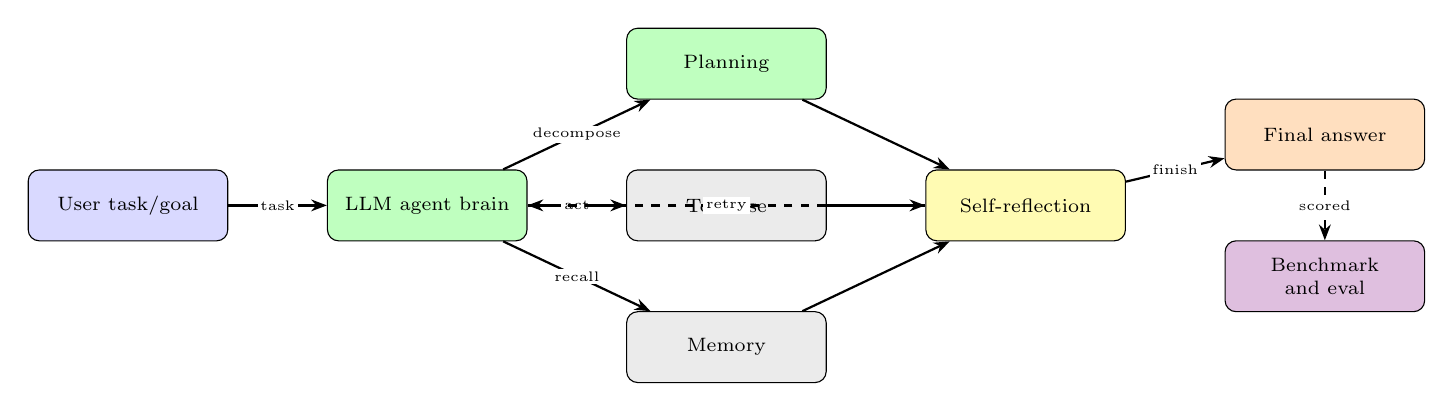
\begin{tikzpicture}
    \node[kuser] (user) at (0.00,0.00) {User task/goal};
    \node[kagent] (agent) at (3.80,0.00) {LLM agent brain};
    \node[kagent] (plan) at (7.60,1.80) {Planning};
    \node[kdata] (tools) at (7.60,0.00) {Tool use};
    \node[kdata] (memory) at (7.60,-1.80) {Memory};
    \node[kdecision] (reflect) at (11.40,0.00) {Self-reflection};
    \node[koutput] (output) at (15.20,0.90) {Final answer};
    \node[kguard] (eval) at (15.20,-0.90) {Benchmark and eval};
    \draw[flow] (user) -- (agent) node[midway, font=\tiny, fill=white, inner sep=1pt]{task};
    \draw[flow] (agent) -- (plan) node[midway, font=\tiny, fill=white, inner sep=1pt]{decompose};
    \draw[flow] (agent) -- (tools) node[midway, font=\tiny, fill=white, inner sep=1pt]{act};
    \draw[flow] (agent) -- (memory) node[midway, font=\tiny, fill=white, inner sep=1pt]{recall};
    \draw[flow] (plan) -- (reflect);
    \draw[flow] (tools) -- (reflect);
    \draw[flow] (memory) -- (reflect);
    \draw[flow, dashed] (reflect) -- (agent) node[midway, font=\tiny, fill=white, inner sep=1pt]{retry};
    \draw[flow] (reflect) -- (output) node[midway, font=\tiny, fill=white, inner sep=1pt]{finish};
    \draw[flow, dashed] (output) -- (eval) node[midway, font=\tiny, fill=white, inner sep=1pt]{scored};
  \end{tikzpicture}%
  }
  \end{center}
  \begin{center}\scriptsize How an LLM agent turns a user goal into an answer, and where evaluation measures each step.\end{center}
\end{frame}
\note{This diagram shows the loop we're actually evaluating. A user gives the agent a goal, and the LLM acts as the brain. It plans, calls tools in its environment, and uses memory. Crucially, it can reflect on its progress and loop back to fix mistakes before giving a final answer. The evaluation harness on the right watches all of this and scores both the result and the steps.}
\begin{frame}[allowframebreaks]{How It Works (Explained)}
\begin{itemize}
  \item A user hands the agent a goal, such as fix this software bug.
  \item The LLM agent is the brain that decides what to do next.
  \item It plans steps, calls tools in an environment, and reads or writes memory.
  \item Self-reflection checks progress and can loop back to retry failed steps.
  \item When satisfied, the agent returns a final answer or action.
  \item An evaluation harness scores both the output and the full step-by-step trajectory.
\end{itemize}
\end{frame}
\section{Example Walkthrough}
\begin{frame}[allowframebreaks]{Example Walkthrough: Example: A coding agent solving one SWE-bench issue}
\begin{enumerate}
  \item The agent receives a real GitHub issue describing a software bug.
  \item It plans: locate the faulty file, understand the code, then edit it.
  \item It uses tools to search the repository and read relevant source files.
  \item It writes a code patch and remembers what it changed via memory.
  \item Self-reflection: it runs the tests; if they fail, it revises the patch.
  \item The final patch is submitted as the agent's answer.
  \item SWE-bench runs the project's real unit tests to score pass or fail.
\end{enumerate}
\end{frame}
\note{Let's make it concrete with one coding example. Imagine the agent gets a real bug report from GitHub. It plans where to look, searches the code, writes a fix, and remembers what it changed. Then it runs the tests; if they fail, it tries again. Finally, SWE-bench runs the project's real tests to decide pass or fail. That's an agent working end to end.}
\section{Results}
\begin{frame}[allowframebreaks]{Results / Findings}
\begin{itemize}
  \item The survey delivers the first comprehensive map of LLM agent evaluation.
  \item SWE-bench evaluates coding agents on 2,294 real GitHub issues via unit tests.
  \item GAIA offers 466 assistant questions across three rising difficulty levels.
  \item WebArena provides 812 realistic web tasks scored by functional success.
  \item tau-bench tests conversational agents in retail and airline customer service.
  \item Evaluation is shifting toward realistic, continuously updated live benchmarks.
\end{itemize}
\end{frame}
\note{So what did the survey find? Mainly, it delivers the first complete map of this field. Along the way it catalogs benchmarks like SWE-bench with its 2,294 real bugs, GAIA with 466 questions across three levels, and WebArena with 812 web tasks. The big trend is a clear shift toward realistic, constantly updated tests so agents can't just memorize answers.}
\section{Discussion}
\begin{frame}{Discussion}
\begin{itemize}
  \item Benchmarks are moving from toy tasks to messy, real-world environments.
  \item A single success rate hides why an agent failed; step-level analysis helps.
  \item It matters to separate the LLM's quality from the surrounding agent code.
  \item As agents saturate old benchmarks, tests must keep getting harder.
\end{itemize}
\end{frame}
\note{Stepping back, a few themes stand out. Benchmarks are getting more realistic and messy, which is good. But just reporting a success rate hides why an agent failed, so step-level analysis matters. And it's important to separate the underlying model's smarts from the code wrapped around it.}
\section{Challenges}
\begin{frame}{Limitations \& Challenges}
\begin{itemize}
  \item Most benchmarks report only final success, not fine-grained skill breakdowns.
  \item Cost and efficiency of agents are rarely measured, though they matter in practice.
  \item Safety, trustworthiness, and policy compliance are under-tested.
  \item Many benchmarks rely on human annotation, which is costly and hard to scale.
\end{itemize}
\end{frame}
\note{The survey is also honest about weaknesses. Most tests only report whether the final answer was right, not which skill broke down. Cost, safety, and robustness are barely measured, even though they're critical in the real world. And relying on humans to label data makes evaluation expensive and hard to scale.}
\section{Future Work}
\begin{frame}{Future Work}
\begin{itemize}
  \item Build fine-grained metrics that reveal exactly where agents go wrong.
  \item Add cost, latency, and efficiency to standard agent evaluation.
  \item Develop stronger safety and robustness tests before real-world deployment.
  \item Create scalable, automated, continuously updated live benchmarks.
\end{itemize}
\end{frame}
\note{Looking ahead, the authors call for a few things. We need finer-grained metrics that pinpoint exactly where agents fail. We should measure cost and speed, not just accuracy. And we badly need stronger safety tests and automated, continuously refreshed benchmarks.}
\section{Conclusion}
\begin{frame}{Conclusion}
\begin{itemize}
  \item As agents get more capable, trustworthy evaluation becomes essential.
  \item This survey organizes agent evaluation into skills, domains, generalists, and tools.
  \item The field is trending toward harder, more realistic, live evaluations.
  \item Key gaps remain in cost, safety, robustness, and fine-grained scoring.
\end{itemize}
\end{frame}
\note{To wrap up: as agents get more capable, trusting them requires solid evaluation. This survey gives us a clean map of skills, domains, generalists, and tools. The field is heading toward harder, more realistic tests, but real gaps remain in cost, safety, and fine-grained scoring. If you remember one thing, it's that measuring agents well is just as important as building them.}
\section{References}
\begin{frame}[allowframebreaks]{References}
  \footnotesize
  \begin{enumerate}
    \item Yehudai, A., Eden, L., Li, A., Uziel, G., Zhao, Y., Bar-Haim, R., Cohan, A., Shmueli-Scheuer, M. (2025). Survey on Evaluation of LLM-based Agents. arXiv:2503.16416.
    \item Jimenez, C. E., Yang, J., Wettig, A., Yao, S., Pei, K., Press, O., Narasimhan, K. (2023). SWE-bench: Can Language Models Resolve Real-World GitHub Issues? arXiv:2310.06770.
    \item Mialon, G., Fourrier, C., Swift, C., Wolf, T., LeCun, Y., Scialom, T. (2023). GAIA: A Benchmark for General AI Assistants. arXiv:2311.12983.
    \item Zhou, S., Xu, F. F., Zhu, H., et al. (2023). WebArena: A Realistic Web Environment for Building Autonomous Agents. arXiv:2307.13854.
    \item Yao, S., Shinn, N., Razavi, P., Narasimhan, K. (2024). tau-bench: A Benchmark for Tool-Agent-User Interaction in Real-World Domains. arXiv:2406.12045.
    \item Liu, X., Yu, H., Zhang, H., et al. (2023). AgentBench: Evaluating LLMs as Agents. arXiv:2308.03688.
  \end{enumerate}
\end{frame}
\begin{frame}[plain]
  \begin{center}
    {\Huge Thank You}\\[1em]
    {\large Questions?}
  \end{center}
\end{frame}
\end{document}